%v4.4
\subsection{The BigBite Spectrometer}
%
\label{sec:expsetup_bigbite}             
%
Scattered electrons will be detected in the BigBite spectrometer.
The spectrometer consists of a single dipole magnet (with magnetic field approximately $1.2~\mathrm{T}$) and a detection system, see Fig.~\ref{fig:BB}.  

\begin{figure}[htbp]
\begin{center}
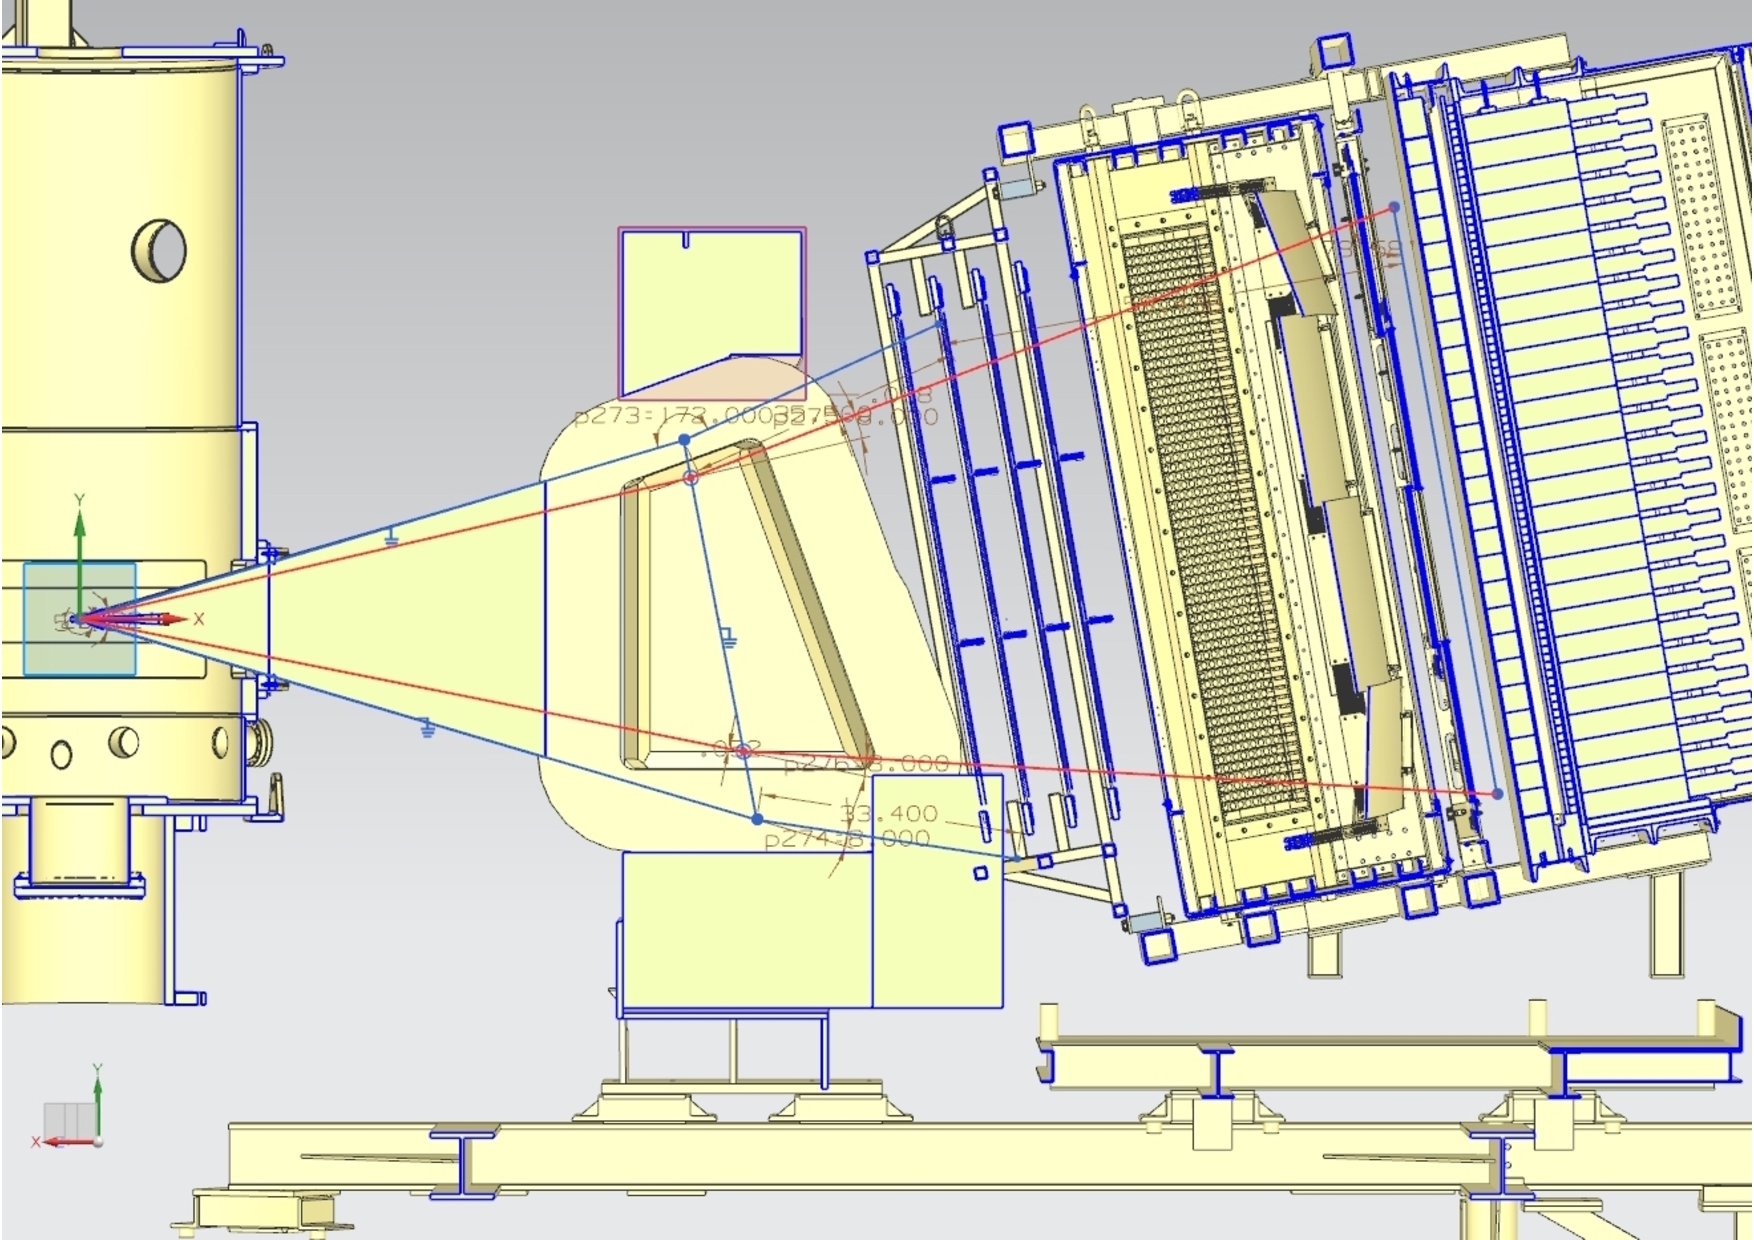
\epsfig{file=Plots/BB_Side-view.pdf,height=3.0in}
\end{center}
\caption{The BigBite spectrometer with the upgraded detector stack.}
\label{fig:BB}
\end{figure} 

\subsubsection{GEM Chambers}
To perform the tracking of charged particles under the high rates anticipated for this experiment, the drift chambers were replaced with gas electron multiplier (GEM) detectors.  
These detectors have proven to be capable of operating under luminosities of $25~\mathrm{kHz/mm}^2$ for the COMPASS experiment at CERN and the spatial resolution of each of these chambers is anticipated to be about $70~\mathrm{\mu m}$.
There will be two sets of GEMs placed on each side of the GRINCH Cherenkov detector.

The set of GEMs in front of the GRINCH is composed of four layers of GEMs.
Two of these layers have been built by will the SBS collaborators from INFN.
They are composed three modules each, measuring $40~\times~50~\mathrm{cm}^2$, such that each layer covers $40~\times~150~\mathrm{cm}^2$ (the long dimension being vertical, along the dispersive direction). The readout of these modules are oriented in the $x/y$ direction {\it i.e.} parallel and perpendicular to the dispersive direction (horizontal and vertical).
The two other layers are being built by the SBS collaborators from UVA. They are composed of a single module measuring $40~\times~150~\mathrm{cm}^2$, the long dimension again being vertical and along the dispersive direction.
The readout of these modules are oriented in the $u/v$ direction {\it i.e.} $\pm~30$~degrees with respect to the horizontal direction.

The set of GEMs behind the GRINCH has been been built by the SBS collaborators from UVA. It is composed of a single layer composed of four modules measuring $50~\times~60~\mathrm{cm}^2$ , such that the layer covers $60~\times~200~\mathrm{cm}^2$ (the long dimension again being along the dispersive direction).
The readout of these modules are all oriented in the $x/y$ direction.

\iffalse
On Fig.~\ref{fig:uva_gem} is displayed the single back GEM layer.
%
\begin{figure}[!h]
  \begin{center}
    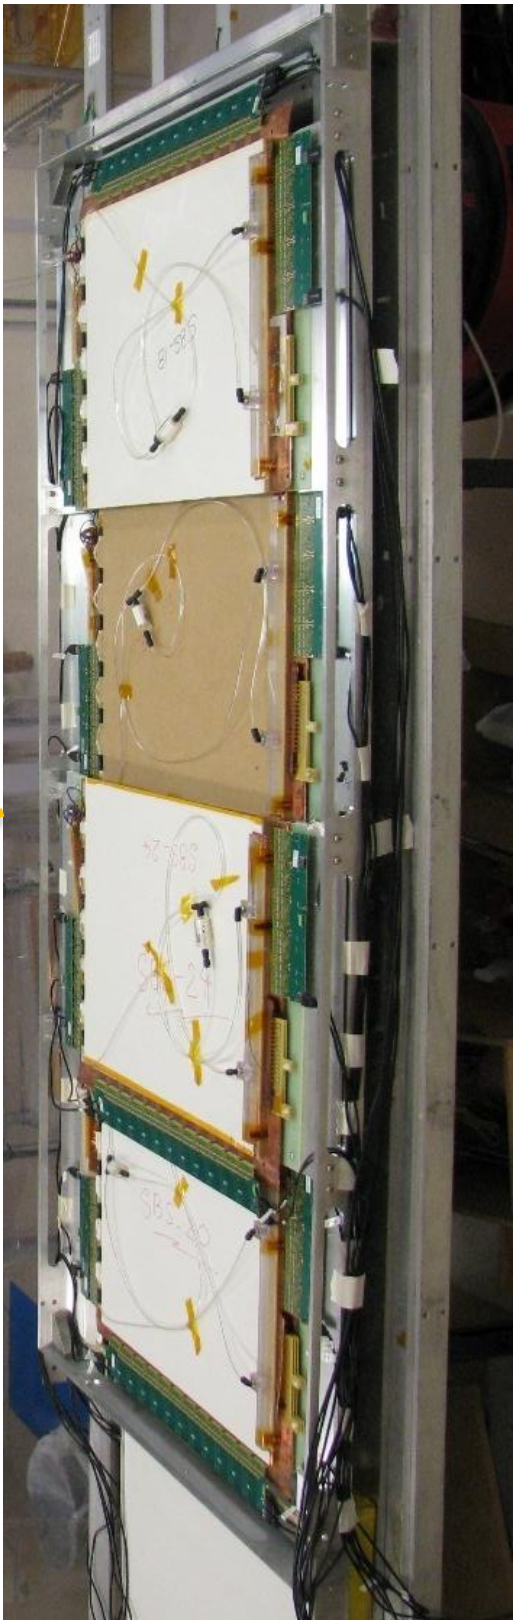
\includegraphics[angle=-90,width=10cm]{Plots/UVaGEMs.png}
    \caption{Picture of the back layer of GEMs, illustrating its arrangment}
    \label{fig:uva_gem}
  \end{center}
\end{figure}
%

For two sets of GEM chambers separated by a distance $z_\mathrm{GEM}$ and including multiple scattering effects, the angular resolution can be approximated by 
\begin{equation}
\left( \delta \theta \right)^2 = \frac{\sigma_x^2}{z_\mathrm{GEM}^2} + \left(\frac{13.6~\mathrm{MeV}}{\beta c p} \sqrt{x/X_0} \left[1+0.038\ln(x/X_0)\right]  \right)^2
\end{equation}
where $\beta c$ is the velocity of the electron, $p$ is the momentum of the electron, and $x/X_0$ is the thickness of the scattering material in radiation lengths.

For small deflection angles from a dipole magnet, the deflection angle, $\theta$, and the momentum, $p$, are related by the equation
\begin{equation}
p = \frac{ e \int B_\perp \cdot dl}{\theta},
\end{equation}
where $\int B_\perp \cdot dl$ is the field integral for the path of the electron.  
For electrons of momentum $3\sim4~\mathrm{GeV}$ and a field integral of $1.0~\mathrm{T\cdot m}$, this would yield a typical momentum resolution of $\delta p/p \approx 0.5\%$.

In order for us to accurately determine the scattered electron's angular
coordinates, momentum, and the position of the scattering vertex along the target, the optics of BigBite need to be studied.  
Data from a multi-foil carbon target and a removable lead sieve located 
at the front face of the magnet provide an accurate method to calibrate the angular coordinates 
before magnetic deflection and a beamline scattering vertex position.  
Data from elastic coincidence $ep$ scattering from a $\mathrm{H_2}$ target will provide data to calibrate the electron momentum and will be performed for each beam energy setting.  
As the kinematics for quasielastic and elastic scattering are similar, this provides the most efficient and reliable method for calibration.  
With the sieve plate in place, it also eliminates the need for $B=0$ field data, which was proven difficult to extract due to prohibitively high rates of otherwise deflected low energy particles.
\fi

The level background in the GEMs have been evaluated, thanks to G4SBS (\cite{g4sbs} abd Sec.~\ref{sec:simu}) for the $G_M^n$ experimental readiness review. % \cite{gmn_err}.
For the $G_M^n$ highest $Q^2$ point (which is the most constraining, since it combines mandatory maximum luminosity and smaller BigBite angles, the background level in the front GEMs are of the order of $120~\mathrm{kHz/cm}^2$ for the front GEM layers, and below $50~\mathrm{kHz/cm}^2$ for the back GEM.
To perform the GEM tracking within such a background environment, we use the cluster reconstructed in the BigBite shower as a track seed to clean the large combinatorics that would otherwise be created by the large number of hits. After this, the main challenge is the separation by the clustering algorithm of the signal and background hits to minimize track smearing.
At this level of background, a TreeSearch tracking algorithm combined with a fairly simple cluster separation algorithm has already proven to achieve 70\% efficiency at nominal luminosity.
A better cluster separation algorithm is currently being developed and should allow to significantly improve this figure. 

\iffalse
\subsubsection{Simulation of BigBite}

Two packages of programs for the simulation of the BigBite spectrometer characteristics
were developed independently by V. Nelyubin \cite{nel01} and S.~Riordan.  
For this experiment, the momentum of the scattered electrons will be approximately $\mathrm{3.5~\mathrm{GeV/c}}$ for the $Q^2 = 10~\mathrm{GeV}^2$ point, 
leading to an expected momentum resolution of $\delta$p/p  of about 0.5\%.  
The expected position resolution on target
along the beam is $\sigma$= 4 mm, and the expected angular resolution in both 
scattering planes is better than $\sigma$=0.3 mrad.  

Additional MC studies were done to evaluate the parameters of the proposed experiment.  
The range of \qsq~accepted by the electron arm is shown in Fig.~\ref{pic:mom_range}. 
The solid angle of the electron arm for different positions along the target is shown in Fig.~\ref{pic:solidangle}.  
The average solid angle for our maximum electron energy is about 44 msr.
%

\subsubsection{Background Rate in BigBite}

Several MC simulations~\cite{pavel} and real data sets~\cite{riordan} were used for the calculation of the 
rate on the BigBite detectors. 
%
Charged particles with momenta below 300 MeV/c
will be deflected entirely out of the acceptance by the BigBite dipole. 
The majority of charged background particles with momentum above 300 MeV/c are $\pi^-$, and for pions near quasielastic 
electron momentum, are about a factor of 3 higher in rate than electrons (Sec.~\ref{sec:bbpion}).  
With an overall pion rejection factor of 10000:1, this number can be reduced to a negligible amount.

The total trigger rate on the shower/preshower with a threshold of $1.7~\mathrm{GeV}$ is expected to be about $2~\mathrm{kHz}$ from a simulation based on pion production rates from a parameterization done by Wiser~\cite{wiser}, Fig.~\ref{pic:rates}.  
This simulation when compared to the previous $G_E^n$ experiment predicted rates higher by a factor of 5, so this produces an upper limit on expected rates.  
Furthermore, adding the Cerenkov into the trigger configuration to explicitly reject pions and photons will be possible if necessary.

A majority of hits in the GEM chambers will be produced by photons.  
To investigate the photon detection probability a separate GEANT-4 code was used. 
The GEM geometry and materials were chosen to be the same as in the COMPASS chambers.
The probability to produce a secondary electron in the drift gap of the chamber as a function
of the energy of the initial soft photon is shown in Fig.~\ref{pic:gemphotons}. It is about $10^{-3}$ at 100 keV and
increases up to $4\times10^{-3}$ at 1 MeV. 
Above 1 MeV the photon efficiency (Fig.~\ref{pic:gemphotons2}) increases but doesn’t exceed 1\%. In the same figures, bottom panels, the probability for correlated
hits in two or more chambers is shown. 
This happens when one photon produces secondary electrons in several chambers. 
One can see that such a probability is negligible for photon energies below 1 MeV, and the hit rates on the chambers are dominated by uncorrelated
random hits.

Using data from the Transversity experiment, E06-010, which placed BigBite at $30^\circ$ at
$1.5~\mathrm{m}$ with a beam current of $12~\mathrm{\mu A}$, the rate per $140~\mathrm{cm}\times35~\mathrm{cm}$ chamber was $41~\mathrm{MHz}$.  
At our beam energies, beam current, active area, target length, and BigBite distance, we expect an increase in rate by about a factor of 13.  
Estimating the BigBite drift chamber photon efficiency to be at most a factor of 5 smaller than the GEM chambers, 
we anticipate an overall increase in the observed rate in the drift chambers to be a factor of 65, or a rate
of $4.5~\mathrm{kHz/mm^2}$. 
This is below rates in which these have been demonstrated to operate.
Using information from the shower and scintillator, the area in the GEM chambers to search for tracks can be restricted
 by a factor of 10, leading to approximately 26 false hits in a $100~\mathrm{ns}$ time window per plane.  
Current transversity tracking code operates with a time window larger by a factor of three
and without using shower information, presenting an overall background rate the tracking must
contend with higher by only a factor of two.  
This should present no problem for current BigBite tracking software.

Using rates of charged particles above $300~\mathrm{MeV}$, less than 20\% of events are anticipated 
to have multiple tracks in the same region as the triggering track.  
The $x$ and $y$ components of  these tracks can be separated using the fixed $z$ plane positions given by the shower and scintillator plane.
\fi

\subsubsection{Shower/Preshower}

The electromagnetic calorimeter configuration consists of two planes of lead glass blocks which  which we call the preshower and shower.  
The preshower, located about $80~\mathrm{cm}$ behind the first GEM chamber, consists of a $2\times26$ plane of $37~\mathrm{cm}\times 9~\mathrm{cm}$ blocks.  
The shower, about $1~\mathrm{m}$ behind the first GEM chamber, consists of an $7\times27$ array of $8.5~\mathrm{cm}\times8.5~\mathrm{cm}$ blocks.  Sums over these blocks form the physics event trigger for the experiment.

The preshower signal can be used to provide an additional method of pion rejection.  
By selecting low preshower signals, a pion rejection factor of 1:50 can be achieved through optimization.  
Despite higher particle rates, pion rejection performance is anticipated to be similar to that achieved for Transversity, E06-010.  
By measuring the pedestal widths and resolution for E06-010 and scaling to this proposal's conditions, overall relative energy resolution for the detector is expected to become worse by a factor of $1.6$, to about $\sigma_{\delta E/E} = 25\%$.

\subsubsection{Timing hodoscope}

The BigBite timing hodoscope has been built the the SBS collaborators from Glasgow, to replace the BigBite scintillator plane.
It will be composed of 90 bars stacked in a plane, each with dimensions $1~\mathrm{in.}\times1~\mathrm{in.}\times60~\mathrm{cm}$. The paddle stack will be oriented such as the long dimension of the bars is horizontal {\it i.e.} perpendicular to the dispersive direction.
Each of these elements are readout by a PMT on each side, mostly to provide measurement redundancy.

\iffalse
The arrangement of these elements can be visulaized on Fig.~\ref{fig:hodo}
%
\begin{figure}[!h]
  \begin{center}
    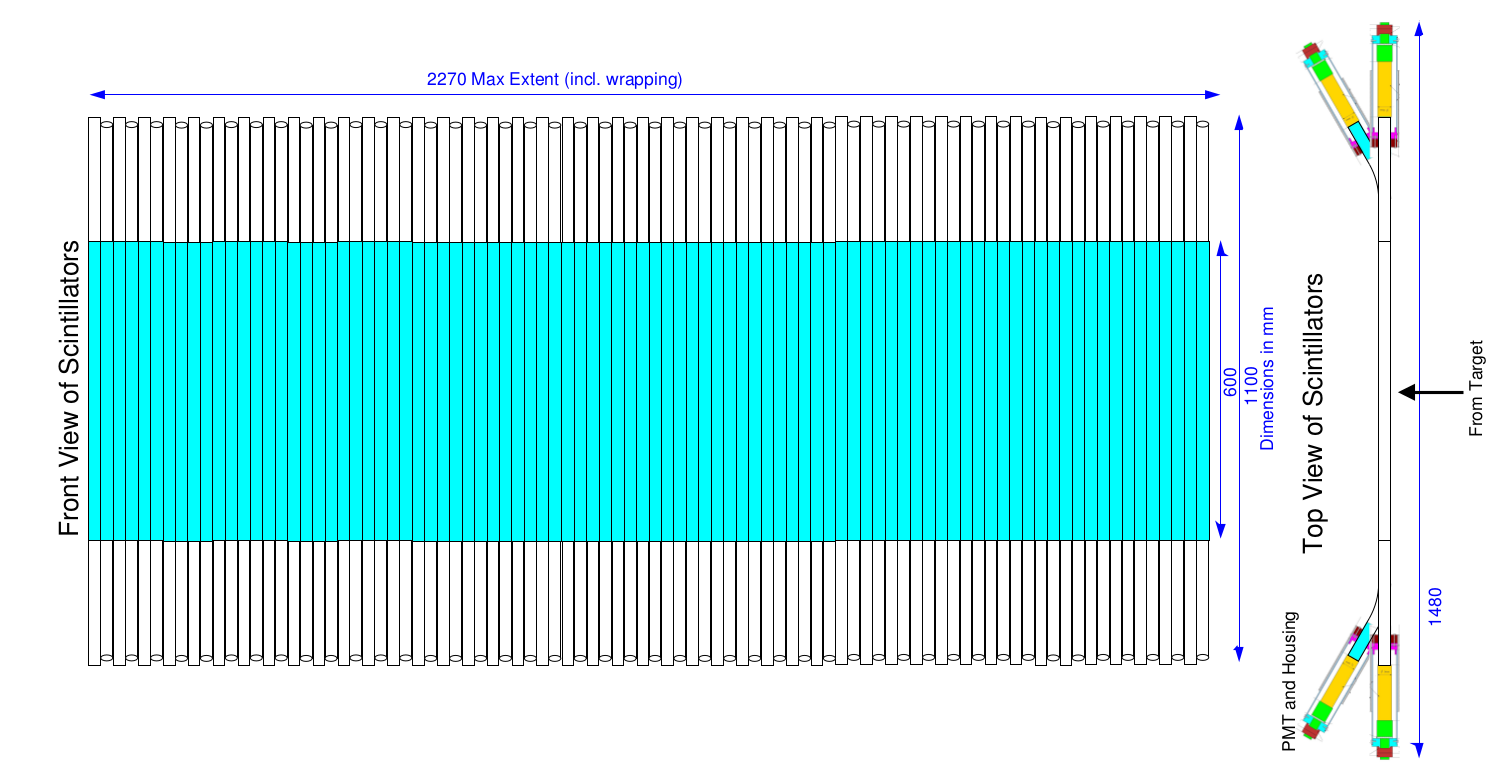
\includegraphics[angle=-90,width=5cm]{Plots/Hodo.png}
    \caption{Arrangement of the timing hodoscope elements.}
    \label{fig:grinch}
  \end{center}
\end{figure}
%
\fi
This plane will primarily be used to provide a signal for nucleon time of flight reconstruction. A time resolution of $200~\mathrm{ps}$ is anticipated.
%For the transversity experiment, where BigBite is at $30^\circ$ using a shorter $40~\mathrm{cm}$ \he~target, and $12~\mathrm{\mu A}$ beam, the rate
This fine segmentation is meant to lower the rates in the detector. Background studies made for the $G_M^n$ experimental readiness review %\cite{gmn_err}
demonstrated that the rates experienced by each element was $\leq~500~\mathrm{kHz}$ at a luminosity of $2.8~\times10^{38}~\mathrm{cm}^{-2}~\mathrm{s}^{-2}$. %for for the scintillator plane was approximately $3.6~\mathrm{MHz}$.
%Using this data to provide upper limits on the rates seen for our experiment, scaling to current, a longer target, and bar active area, we anticipate a rate of $270~\mathrm{kHz}$ per bar.  
The PMTs pulses are processed by NINO front-end cards which, when the PMT pulse crosses the NINO threshold, will produce a digital signal to be readout by CAEN 1190 TDCs which record a leading time and a trailing time.

\subsubsection{GRINCH cherenkov detector}

The main purpose of the Ring Imaging Cherenkov is to provide additional particle identification for offline pion rejection.
The GRINCH consists of a tank with a maximum depth of $88.9~\mathrm{cm}$, with 4 cylindrical mirrors focussing the cherenkov light directly onto a 510~PMT array (60 lines of PMTs, with lines of 9~PMTs alternating with lines of 8~PMTs) placed away from the beam.
\iffalse
The GRINCH tank and PMT matrix are represented on Fig.~\ref{fig:grinch}
%
\begin{figure}[!h]
  \begin{center}
    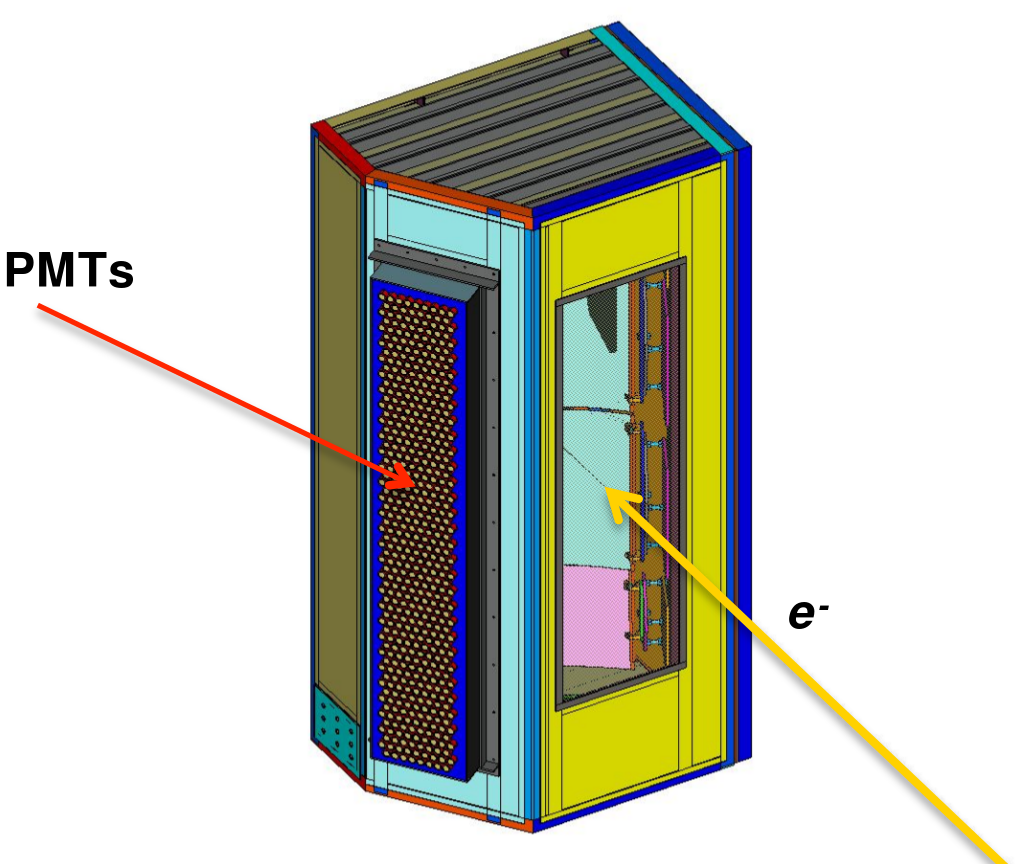
\includegraphics[width=6cm]{Plots/GRINCH.png}
    \caption{CAD representation of the GRINCH tank and PMT matrix}
    \label{fig:grinch}
  \end{center}
\end{figure}
%
\fi
The radiation gas will be $C_4F_8$, which is by far the best compromise between light yield for electrons and operating cost.
With $n-1=1.35\times10^{-3}$, the $\pi$ threshold is only about $2.7~\mathrm{GeV}$, so the additional pion rejection will be most effective below this threshold. 

As for the timing hodoscope The PMTs pulses are processed by NINO front-end cards which, when the PMT pulse crosses the NINO threshold, will produce a digital signal to be readout by VETROC TDCs, which for each PMT hit will record a leading time and a trailing time.
The analog signal will not be recorded however, which means that for each PMT hit, the information of the number of not directly available (although it can in theory be deduced from the time over threshold).

All of this implies that the electron selection relies on the number of GRINCH PMT firing, instead of relying on the signal amplitude.
%Fig.~\ref{fig:GRINCH_rej} shows the rejection 
%Nonetheless, at the kinematics considered, the GRINCH helps reject {\em at least} 60\% of pion background (see Fig.~\ref{}), which, combined with
%
%\begin{figure}[!h]
%  \begin{center}
%    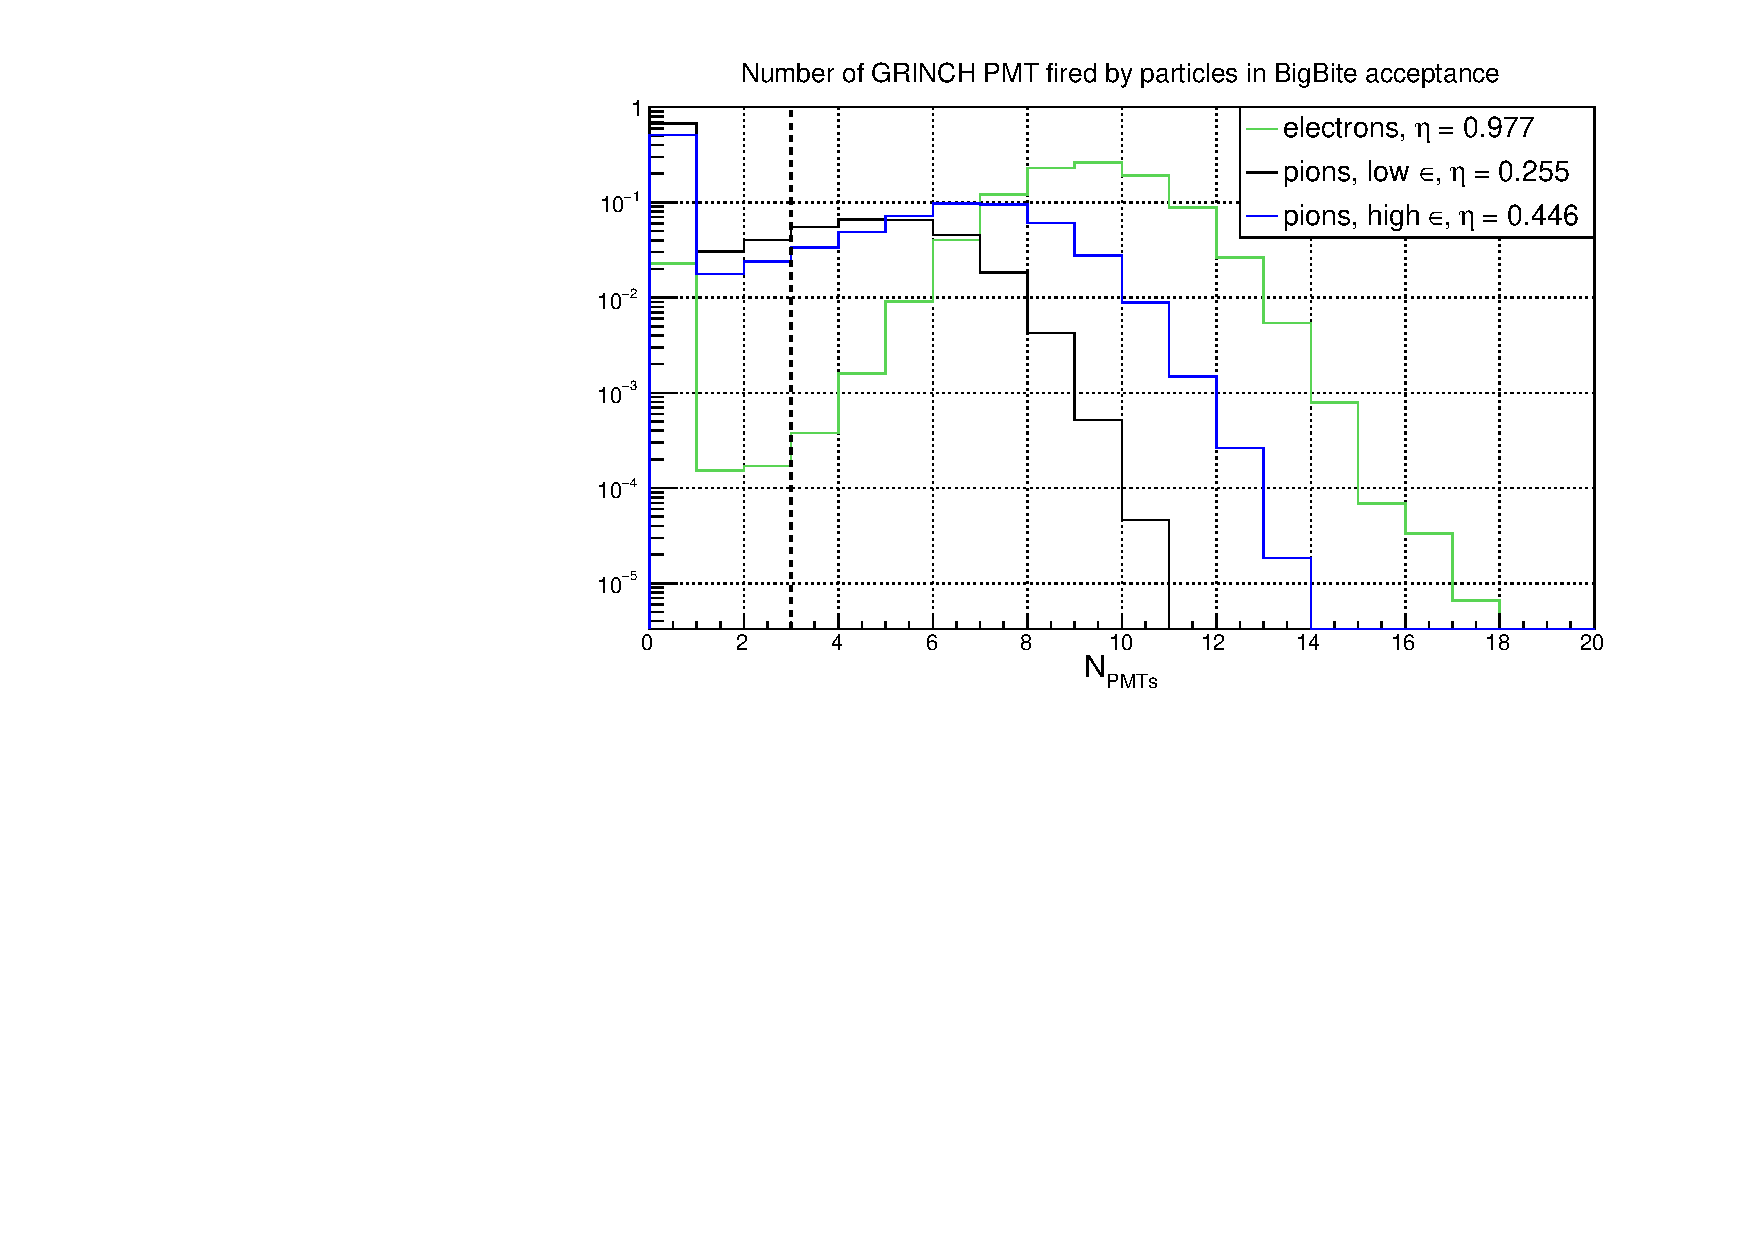
\includegraphics[width=6cm]{Plots/GRINCH_rejection.pdf}
%    \caption{GRINCH response for electrons (green), pions at the low $\epsilon$ kinematic ($k' = 2.0$)}
%    \label{fig:GRINCH_rej}
%  \end{center}
%\end{figure}
%



%For $12~\mathrm{GeV}$ running, to provide a pion threshold of $3.5~\mathrm{GeV}$, a combination of about $50\%$ $\mathrm{CO}_2$, $50\%$ Freon-12 will be used.

%For our conditions, the rate of electrons will be about $30~\mathrm{kHz}$, which in a $100~\mathrm{ns}$ gate will lead to a $0.3\%$ chance of a pion being misidentified by an accidental electron.  
%Using standard calculations, for a charged pion near threshold, there is a $0.1\%$ chance of producing a $\delta$ electron above threshold.  
%Combined, a pion rejection factor from the Cerenkov will be about 1:250, near specifications.  
%Combined with a rejection factor of 1:50 for the preshower provides a $10^4$ overall rejection.
